\chapter{Design and Implementation}
\label{chap:cran_for_lora}

In this section we will be elaborating and reasoning the design decisions taken in order to materialize the idea of IoT based surveillance with the blockchain technology. In the first part we will be discussing in detail the different approaches, technologies and communication protocols considered throughout the design decisions. We will also see how the IoT surveillance system with access control drives the design decisions. 

In the second part the design decisions taken will be put into action by implementing the architecture. A number of APIs and data structures are used to materialize the idea however still the Esp Eye device comes with limitations such as the max array size and due to which a dynamic memory allocation is needed.  





\section{Hardware Components}

Before digging deeper in this section we would like to describe the hardware architecture and its components involved in the project.
The video surveillance for face detection and recognition is handled by ESP EYE where the testing environment is based on an AMD Processor machine which can be Windows/Linux/Mac.
In Figure~\ref{fig:hardarchitecture} on the left hand side we have multiple Esp devices which communicate with the IoT gateway within the same network with Wi-Fi based on IEEE 802.11 standards for communication protocols. 

\begin{figure}[!htb]
    \centering
    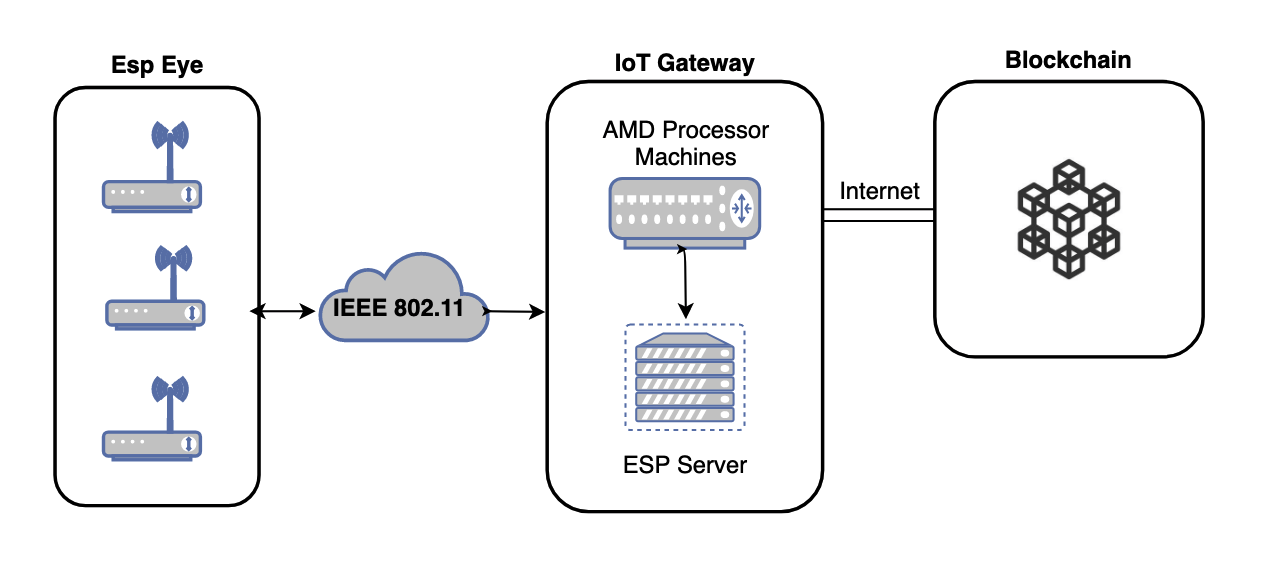
\includegraphics[width=1\textwidth]{figures/Hardware_architecture.png}
    \caption{Hardware Architecture}
    \label{fig:hardarchitecture}
\end{figure}


The IoT Gateway serves as the middle man which waits for images coming from Esp Eye to be inserted into the blockchain. As the main experimental devices in our project we have Esp Eye and the raspberry Pi. But due to experimental purposes we had to run the blockchain locally and that lead us to change the infrastructure and instead of the raspberry pi which is an ARM based processor machine we had to go for AMD based processor machine. This is due to the Hyperledger Fabric which runs in form of containers and its binaries are only available for an AMD processor. However the architecture in the Figure~\ref{fig:hardarchitecture} still holds true. 


\subsection{Esp Eye for Face Detection}

ESP EYE which can be seen in Figure~\ref{fig:espeye} is an AI development board which is based on ESP32 chip. The device was first for sale in 2020 by the semiconductor company Espressif. There are many other devices which are based on the ESP32 family of chips. ESP32 is combine with extra components such as programming interfaces, different sensors which are used for the evaluation of the chip. 
At the core of the board is the dual core Tensilica LX6 processor with 8 MB PSRAM and a 4MB flash. 

The Esp Eye integrates an embedded microphone and a camera with 2-Megapixels. The camera is an OV2640 sensor with a maximum image size of 1600×1200 pixels. The board supports  2.4 GHz Wi-Fi technology to connect to internet through a wide area network. A Micro USB port provides the power supply and also debugging in order to use the AI APIs. It comes with an UART Chip which enables asynchronous serial communication with which the program is uploaded bits by bits. 
\begin{figure}[!htb]
    \centering
    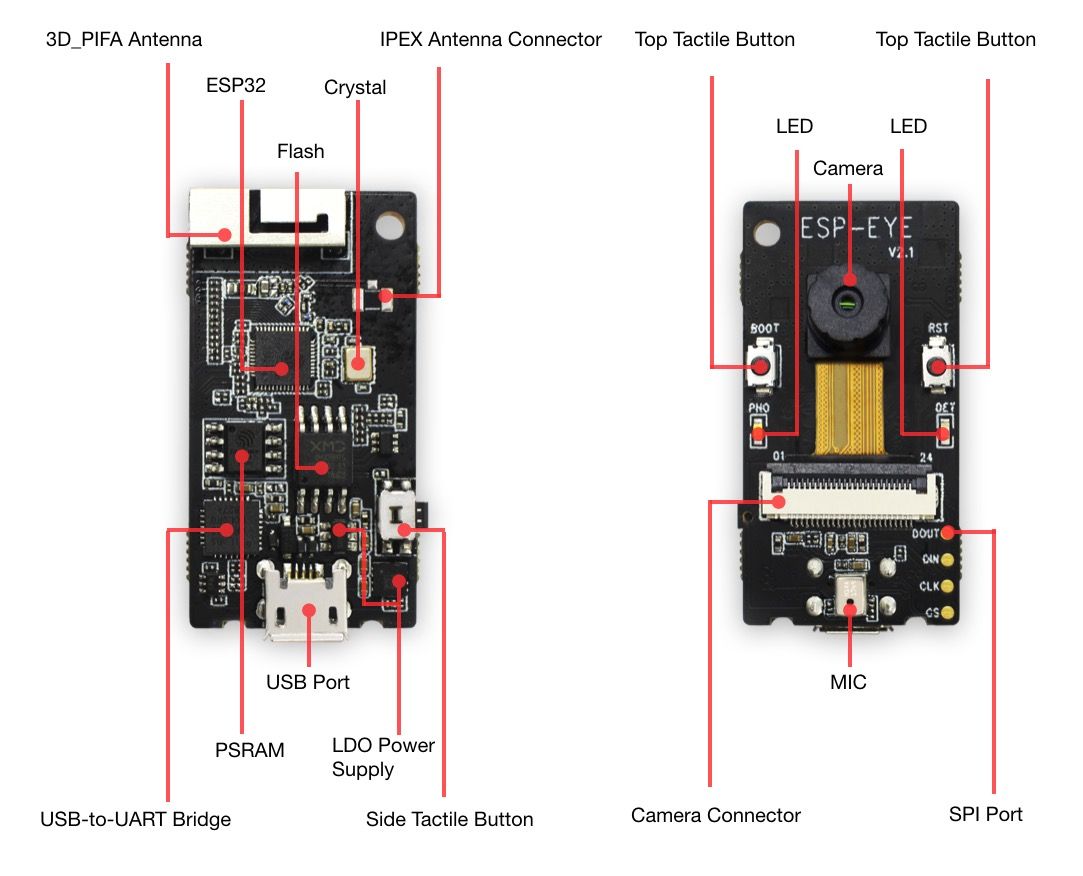
\includegraphics[width=1\textwidth]{figures/espeye.png}
    \caption{Esp Eye}
    \label{fig:espeye}
\end{figure}


Esp Eye also supports additional security features: flash encryption feature and secure boot. The flash encryption is intended to secure the content of the flash memory. In Esp Eye flash encryption is done using AES-256 and the key is stored in the eFuse. eFuses keep the values intact and can not be changed by a software. Since the data in flash is encrypted upon reboot the physical readout will be impossible. 
On the other hand secure boot can protect the device from uploading unsigned code. The algorithm is a typical digital signature method with RSA, the public is stored in the device itself whereas the private is kept secret and used upon each code upload. 

What makes the Esp Eye stand out of the crowd is its performance and the platform for face detection and recognition known as Esp-Who. Esp-who comes with algorithms for face detection and recognition which makes it possible to run both in Esp Eye.

\subsection{Raspberry PI}

Raspberry Pi has been the development environment from the beginning of the project. It is very lightweight, supports many compilers and makes it ideal for experimental purposes. Throughout this project we have been using Raspberry Pi 4 Model B, with 8GB of RAM with  integrated 802.11 wireless LAN. It worth mentioning that the Raspberry Pi is backed by an ARM processor. 
The esp32 family of devices are natively compiled and developed by the esp idf development platform.  Similarly also the Esp-Who libraries for face detection and recognition were available in esp idf development platform.
However after many tries to setup Hyperledger Fabric in Rasperry Pi we realized that Hyperledger Fabric binaries were not possible to run in ARM processor. Therefore after that a computer with AMD processor was used. 






\section{Design}

 


\subsection{Surveillance System Architecture}

Figure~\ref{fig:surveillance2} shows a high level overview with the sotware components. It is important to mention that the design is compatible without any technological restrictions. At the beginning there were two approaches in mind: deployment of face detection and recognition on the cloud or deployment in the Esp Eye device itself. In the first approach AI is deployed on the cloud which means the camera consequently captures images and send them on the cloud for face recognition. This approach is costly, based on the previous studies in average the time required to detect a person is between 2 to 5 seconds. In addition it requires substantial amount of bandwidth which would be wasted if no one is present.

In the second approach which we decided to implement the face detection and recognition run on the IoT device itself. This approach has a lot more benefits, first of all the images are captured by a very small devices powered by AA batteries. Compare to the previous approach they needed a machine on the cloud and a separate camera, whereas in this case both are converged into one single low powered device. When images are captured they are immediately detected and recognized. Which means that it can also be optimized to delete images when a face is not detected. 



\begin{figure}[!htb]
    \centering
    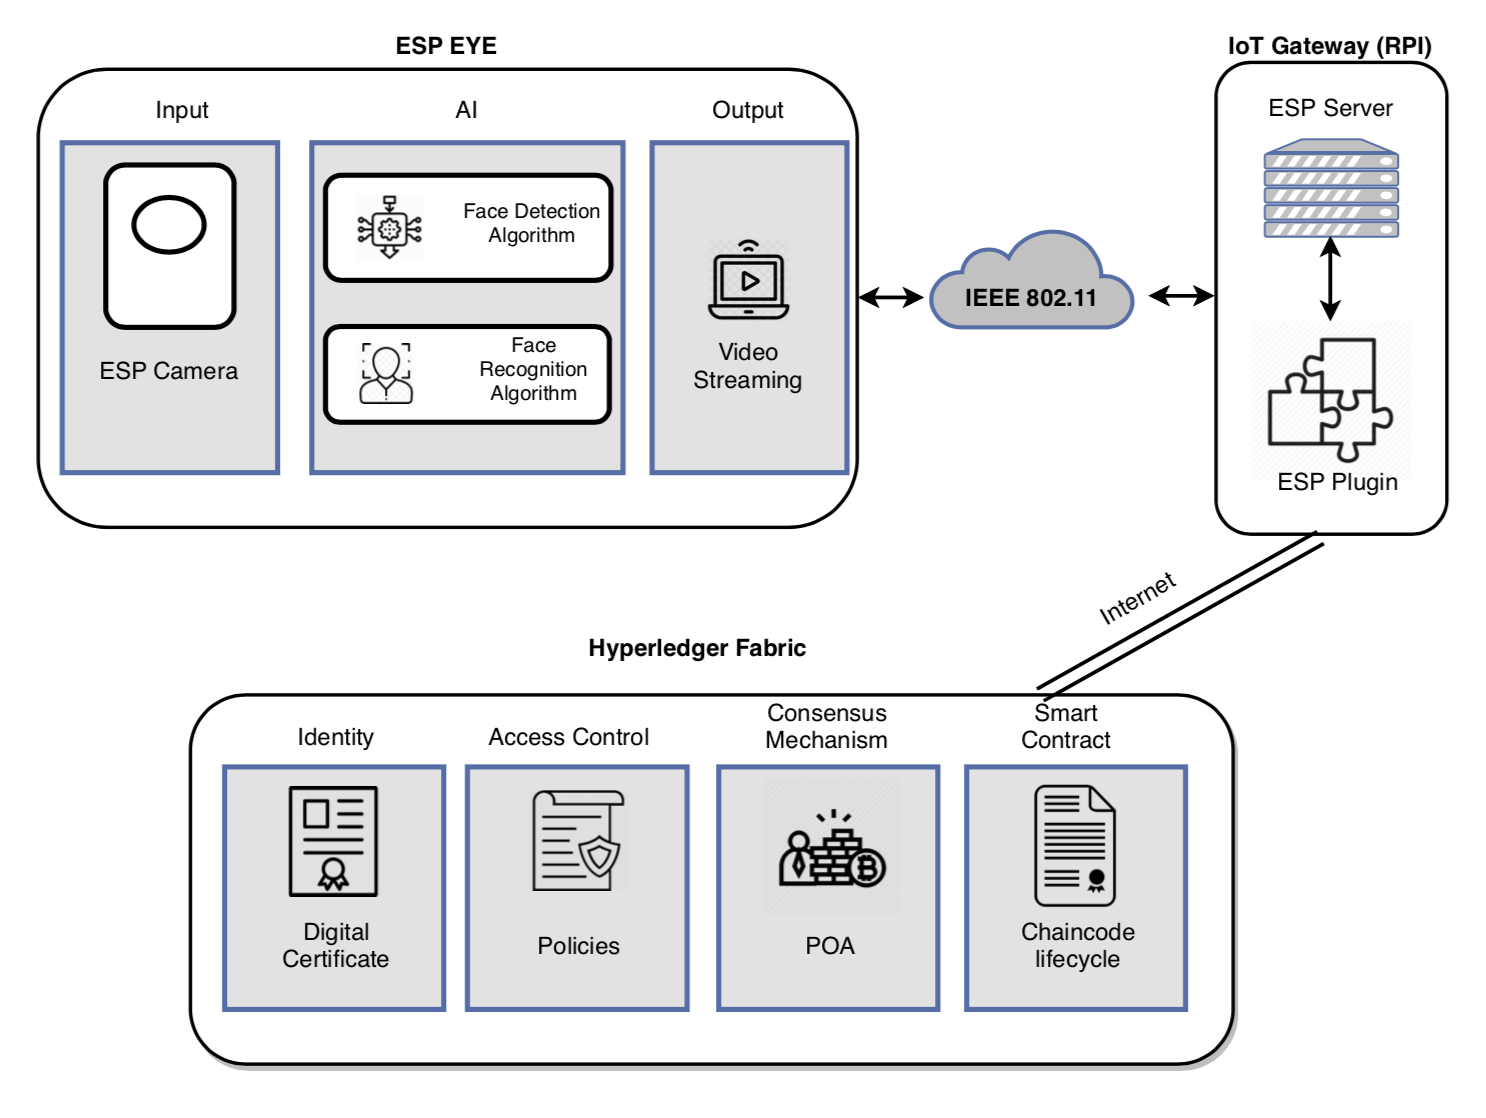
\includegraphics[width=1\textwidth]{figures/esp2.png}
    \caption{Software Architecture}
    \label{fig:surveillance2}
\end{figure}


On the right hand side of the Figure~\ref{fig:surveillance2} is the IoT Gateway which serves as a hub to do the rest of the job. The communication between the Esp Eye and the IoT gateway is achieved with a wireless communication compliant to IEEE 802.11 LAN protocols. It follows the client-server architecture, the Esp Eye is the client and the IoT Gateway as a server. Since we want to store the detected images in the blockchain having the Esp Eye as a client fulfills the requirements. The server will be waiting for requests coming from the Esp Eye. The other way around would not work, since the only way to send data from the server is when the client has sent a request. The first condition for the image to be stored in blockchain is that the face has to be detected in that image. On the other hand ESP Plugin with the help of the SDK from Hyperledger Fabric will start the process of submitting the transaction to the ledger. Hyperledger Fabric enables the storage of the detected images coming from the Esp Eye.   

\subsection{Communication Protocols under consideration}
When it comes to decision which communication protocol to use in IoT device, it is important to go for a lightweight protocol and among our choices is HTTP and MQTT both of them supported by Esp Eye with the help of IPEX antenna which enables the Wi-Fi connectivity. MQTT is an extreme lightweight protocol which follows the publish/subscribe model for communication. Whenever a client pushes a message on a subscribed topic then the message will be forwarded to all the clients participating on that topic. Due to the use case where the esp eye devices do not have to communicate in between the MQTT leaves behind. 
Instead HTTP protocol is employed where Esp Eye and the IoT Gateway communicate in the client server architecture respectively. For the inter-machine communication the REST architectural style will be used because anyways we do not want to bind the communication since we do not know when the face will be detected. Besides REST is considered to be more lightweight compare to its counterparts. For the data-interchange format the JSON format is employed which is very lightweight and performs much better since its syntax follows the javascript language so it makes it faster to read since the ESP server is also written in javascript.  
\subsection{Face detection and recognition in sensor node}
ESP WHO Platform, talk about the algorithm a little bit




\subsection{Hyperledger Fabric a tamper-resistant database}

  The main criteria were that the blockchain ought to be private and permissioned since the images should not be public and only available from within the organisation that applies our use case. Ethereum and Hyperledger Fabric was another potential candidate to be deployed.Among the two we decided for Hyperledger Fabric because from the beginning it is meant to be private permissioned blockchain. Although Ethereum can be adapted to serve our needs but yet it comes with a consensus mechanism which is energy demanding and not flexible. Hyperledger Fabric provides a modular architecture and enables more flexibility and is tailored to the needs of our use case. For a better undestanding of the architecture of Fabric you can refer to Chapter 4.  Hyperledger Fabric in our case stands out of the crows due to its features: 

\begin{itemize}
    \item High transaction throughput
    \item Low latency for transaction confirmation
    \item Confidentiality of transactions with the help of channels
    \item Highly modular architecture
    \item Identities supplied with digital certificate 
\end{itemize}

With its modular architecture it allows to be tailored to the needs and the use case. It has been designed to be highly configurable and offers modularity for the following components: 

\begin{itemize}
    \item A pluggable consensus or ordering service which is the core component for transection execution.
    \item A pluggable Membershi Service Provide responsible for managing entities and associating them with cryptographic information.
    \item A pluggable Certificate Authority responsible for issuing and managing the identities with digital signature cryptography.
     \item A smart contract implemented in a conventional programming languages known to developers. 
    
\end{itemize}



\section{Implementation}
\subsection{Data Flow Overview}
include data flow diagram

\subsection{Communication Protocol}
\subsection{Implementation Platforms}

ESP IDF
ARDUINO



\section{Results}








